\chapter{Methodology}

As illustrated in Fig. \ref{fig:tikz_methodology}, we have our initial dataset that we split in :
\begin{itemize}
    \item a \textbf{validation set} (10 \% of the dataset) used for hyper-parameter optimization or model selection for localisation and classification
    \item a \textbf{train / test set} (remaining dataset) used for the localisation and classification
\end{itemize}

\begin{figure}[h]
    \centering
    \tikzstyle{block} = [rectangle, draw, text width=3cm, text centered, rounded corners,  fill=blue!20]
    \tikzstyle{line} = [draw,thick, -latex']
    \tikzstyle{cloud} = [draw, ellipse, text width=3cm, text centered]
    \tikzstyle{edge from parent}=[->,thick,draw]
    \begin{tikzpicture}[auto, edge from parent fork down]
        % Distance between node
        \tikzstyle{level 1}=[sibling distance=80mm,level distance=10ex]
        
        % Place nodes
        \node [cloud, fill=red!10] (base) {Dataset}
        child{node [cloud, fill=green!10] (validation) {Validation set}
            child{node [block, fill=blue!10] (hyperparameter) {Hyper-parameter optimization}}
        }
        child{node [cloud, fill=green!10] (train_test) {Train / test sets}
            child{node [block, fill=blue!10] (localisation) {Localisation}
                child {node[block, fill=blue!10](feature){Feature description}
                    child {node[block, fill=blue!10](classification){Classification}
                        child {node[block, fill=red!10](result){Result}
                        }
                    }
                }
            }
        };
        % Draw edges
        \path [line] (hyperparameter.east) -- (localisation.west);
        \path [line] (hyperparameter.south) -- (classification.west);
    \end{tikzpicture}
    \caption{General process of the localisation and classification}
    \label{fig:tikz_methodology}
\end{figure}

\section{Hyperparameter optimization}

There are numerous parameters that are part of the machine learning but are not learnt. Typical example include which kernel function used (if any) or the value of the penalty parameter $C$ for SVM, the number of $k$ of neighborhoods for kNN.

We use the exhaustive grid search method to select the parameters that have the highest performance score through 10 fold cross validation. It generates all the possible combination of parameters value and train / test the classifier.

\section{Localisation}

For localisation, a different approach from the litterature has been used. The usual way is to detect area of food and non food in a picture. Yet, it was noticed that the food items of UEC FOOD 256 and 100 tends to be in the middle and stands out. Moreover, demanding the user to take pictures that follow these charastetics is reasonnable.

That's why a pre-trained CNN used for saliency detection has been used. It has been pre-trained in \cite{zhang2015SOD} on multiple datasets (Multi-Salient-Object, ). It is available \footnote{\url{https://gist.github.com/jimmie33/339fd0a938ed026692267a60b44c0c58}}.

The CNN structure is a copy of \enquote{GoogleNet} model \cite{Szegedy2015}, i.e. it is composed of 22 layers, corresponding to a succession of convolutional, max pooling and activation layers, the last one being a sigmoid funciton.

The CNN has been pre-trained to detect the likelihood to belong to one of the 100 arbitrary bounding boxes as presented in Fig. \ref{fig:seg_100_bboxes}.

\begin{figure}
    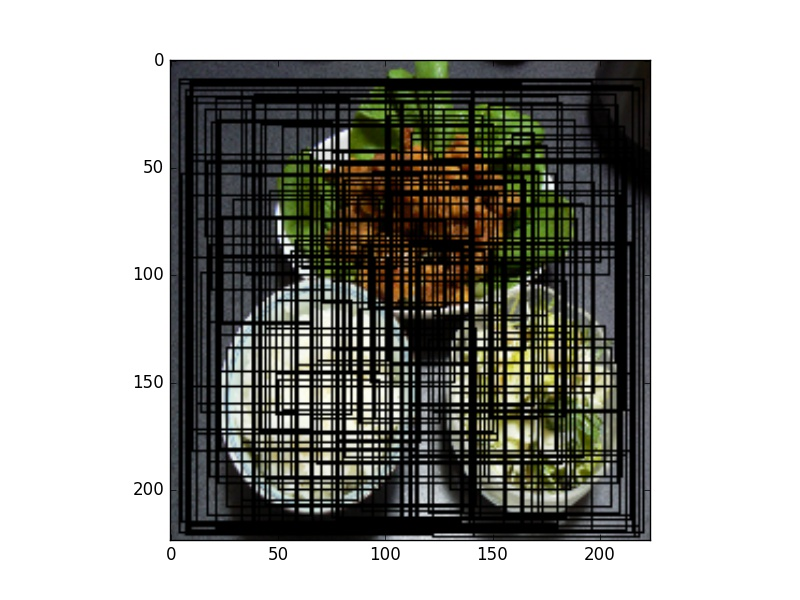
\includegraphics[scale=0.5]{img/seg_100_bboxes.jpg}
    \caption{Picture of the 100 possible bounding boxes that the salient CNN will try to recognise}
    \label{fig:seg_100_bboxes}
\end{figure}


\section{Classification}

\subsection{Histograms and moments}

The first feature descriptor used combined histograms of LBP and Color with color moments for each picture:
\begin{enumerate}
    %\item extract the sub-image delimited by the bounding box
    %\item resize this sub-image to $224 \times 224$ pixels
    \item extract a 100-bin histogram of local binary pattern on the grayscale image
    \item extract a 30-bin by 30-bin joint color histogram for the channel $H$ and $s$ of the HSV  representation
    \item extract the first two moments of the R, G, B, H, S and Gray channels
    \item extract the 7 Hu moments
\end{enumerate}

The feature vectors are then normalized to have all features centered around zero (mean equal to 0) and have unit variance (equal to 1).

Then, apply multiple classifiers:
\begin{itemize}
    \item decision tree
    \item random forest (made up of 500 trees)
    \item SVM
\end{itemize}

Talk in result: show the best amelioration with hyperparemeter (but in general it only improve it by one or two percents)

\subsection{Bag of words}

The first feature descriptor used combined histograms of LBP and Color with color moments for each picture:
\begin{enumerate}
    \item detection of keypoints using a dense grid (4 spaces)
    \item descriptors: Root SIFT. Root SIFT is a simple variant of SIFT, presented in \cite{Arandjelovic2012}. When the SIFT descriptors as been computed for each keypoints, we apply an element wise square root of the L1 normalized SIFT vectors
\end{enumerate}

Then these feature vectors are clustered using using the k-means algorithm to obtain a 1000-word codebook.

For each picture:
compute the histogram of occurence counts of visual words

Kernel trick: use of a variant of the $\chi^2$ kernel named additive $\chi$-squared kernel presented in \cite{Vedaldi2010}

Then we apply the SVM classifier.

\subsection{CNN as a Descriptor}

A pre-trained CNN used for image recognition on ImageNet Challenge 2014.

\cite{Simonyan2014}

it is available \footnote{\url{https://gist.github.com/ksimonyan/3785162f95cd2d5fee77/}}.

The model is an improved version of the 19-layer model used by the VGG team in the ILSVRC-2014 competition.

\section{Code}

The code is freely available on Github\footnote{\url{https://github.com/bnogaret/food_log}}.

I'm using python 3.5.2 and its scientific stack bas on scipy \cite{Oliphant2007}:
\begin{itemize}
    \item numpy \cite{VanDerWalt2011} for N-dimensional array
    \item pandas \cite{McKinney2010} for the data structure
    \item scikit-image \cite{VanderWalt2014} and opencv 3 \cite{Bradski2000} for some of the image processing algortihms
    \item scikit-learn \cite{Pedregosa2012} for most of the machine learning and caffe \cite{Jia2014a}  for the CNN
    \item matplotlib \cite{Hunter2007} for 2D graph generation
    \item sphinx for the documentation
\end{itemize}
